\documentclass[tikz,border=2pt]{standalone}
\usepackage{amsmath}
\usepackage{pgfplots}
\pgfplotsset{compat=1.18}

\begin{document}
% The geometric power series Σ x^n: its partial sums 1 + x + ... + x^N approach 1/(1-x) on
% (-1,1) and run away outside that interval.
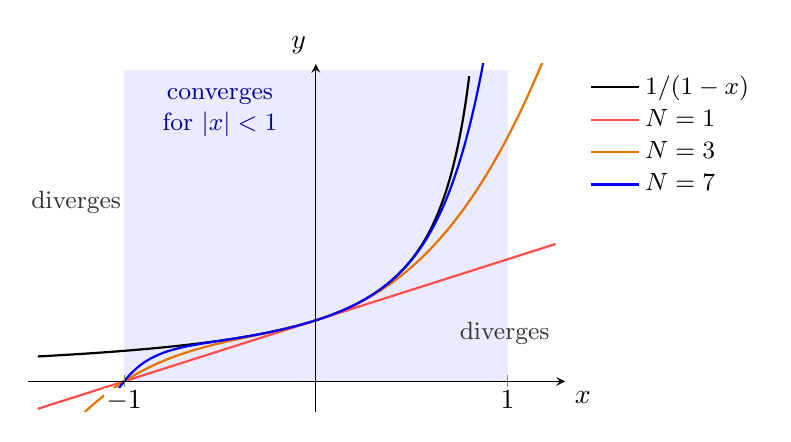
\begin{tikzpicture}
	\begin{axis}[
		axis lines=middle, axis on top,
		xmin=-1.5, xmax=1.3,
		ymin=-0.5, ymax=5.2,
		xtick={-1,1}, ytick=\empty,
		xticklabel style={fill=white, inner sep=1pt},
		xlabel={$x$}, ylabel={$y$},
		xlabel style={below right}, ylabel style={above left},
		samples=160, smooth, clip=true,
		width=8.4cm, height=6cm,
		legend pos=outer north east, legend style={draw=none, fill=none, font=\small}, legend cell align=left
		]
		\fill[blue!8] (axis cs:-1,0) rectangle (axis cs:1,5.1);
		\addplot[thick, black, domain=-1.45:0.8] {1/(1-x)};
		\addlegendentry{$1/(1-x)$}
		\addplot[thick, red!70, domain=-1.45:1.25] {1+x};
		\addlegendentry{$N=1$}
		\addplot[thick, orange!90!black, domain=-1.45:1.25] {1+x+x^2+x^3};
		\addlegendentry{$N=3$}
		\addplot[thick, blue, domain=-1.2:1.22] {1+x+x^2+x^3+x^4+x^5+x^6+x^7};
		\addlegendentry{$N=7$}
		\node[blue!60!black, anchor=north, font=\small, align=center] at (axis cs:-0.5,4.95) {converges\\ for $|x|<1$};
		\node[gray!40!black, anchor=south, font=\small] at (axis cs:-1.25,2.6) {diverges};
		\node[gray!40!black, anchor=south east, font=\small] at (axis cs:1.27,0.45) {diverges};
	\end{axis}
\end{tikzpicture}
\end{document}
